% provavelmente era boa ideia dizer que biliões == mil milhões

\section{Contexto histórico}

\subsection{Origem}     % ver o titulo
Ao contrário de outras aplicações do mesmo estilo, como o \textit{WhatsApp}, que foram criadas sob a alçada de grandes empresas, com um grande financiamento desde o inicio, o \textit{Signal} foi criado como um projeto \textit{open-source} pelo investigador de cibersegurança \textbf{Moxie Marlinspike}. A primeira versão foi lançada em 2014. Desde o inicio que o propósito principal da aplicação é permitir aos seus utilizadores privacidade total quando comunicam usando o serviço, usando para isso um protocolo desenvolvido especialmente para o \textit{Signal}, o \textit{Signal Protocol}, que concede encriptação ponto a ponto ás comunicações feitas.

Apesar do \textit{Signal Protocol} ter sido criado para ser utilizado pelo \textit{Signal}, houve outras aplicações de outras empresas com interesse em usar este protocolo para permitir comunicações seguras sob a sua alçada:

\begin{itemize}
   \item \textbf{\textit{Facebook Messenger}} - Integrada em 2016 o protocolo como uma \textit{feature} adicional para possíveis comunicações mais seguras.
   
   \item \textbf{\textit{Skype}} - Integrada em 2018, como uma nova \textit{feature} em \textit{chats} do tipo \textit{Private Conversations}.
   
   \item \textbf{\textit{WhatsApp}} - Integrada em 2016, sendo que a utilização \textit{default} da aplicação utiliza o protocolo para todas as comunicações. 
\end{itemize}

Sendo que o \textit{Signal} pertence a uma organização sem fins lucrativos (atualmente, \textit{Signal Foundation}), não possui um plano financeiro estável, sobrevivendo de doações feitas por utilizadores e apoiantes da filosofia do serviço. Em 2018, o co-fundador do \textit{WhatsApp}, Brian Acton, doou 50 milhões de dólares à \textit{Signal Foundation} como uma forma de propulsionar o acesso facilitado à possibilidade de realizar comunicações seguras a qualquer cidadão. \cite{history}


\subsection{Presença no mercado}

\subsubsection{Signal}
Sendo que a \textit{Signal Foundation}, tendo como uma das filosofias base a privacidade total dos seus utilizadores, não publica quaisquer dados de utilização da plataforma, nem mesmo o número de utilizadores ativos por intervalo de tempo. Contudo, podemos ter uma noção do número de utilizadores, tendo em atenção o número de \textit{downloads} que a aplicação teve no \textit{Google Play}, de acordo com os dados em 
\cite{signal_android}:

\begin{itemize}
   \item \textbf{Número total de \textit{downloads}}: 20 124 588
   \item \textbf{Número médio de \textit{downloads} diários}: 21 558
\end{itemize}

Para além disso, de acordo com afirmações de Moxie Marlinspike's (fundador do projeto), mais de 40\% dos utilizadores do \textit{Signal} são utilizadores de \textit{iOS}. \cite{signal_ios}

\subsubsection{WhatsApp}
Ao contrário da \textit{Signal Foundation}, o \textit{Facebook} é mais aberto quanto à privacidade dos utilizadores das suas plataformas, sendo que ao longo dos anos tem lançado publicamente estatísticas da utilização do \textit{WhatsApp}. Na figura \ref{graph:whatsapp_monthly_active} é possível analisar o crescimento do número de utilizadores ativos mensais mundialmente desta aplicação.

\begin{figure}[H]
   \begin{center}
       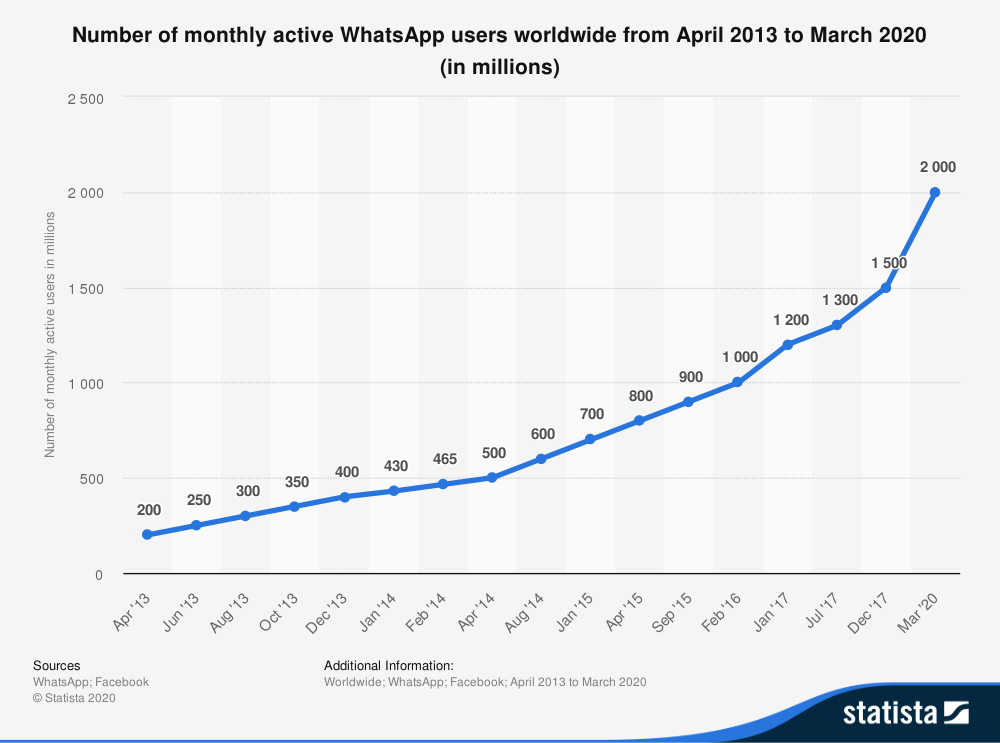
\includegraphics[width=17cm]{img/statistic_id260819_number-of-monthly-active-whatsapp-users-as-of-2013-2020}
       \caption{Número de utilizadores mensais do \textit{WhatsApp} entre abril de 2013 e março de 2020. \cite{whatsapp_monthly_users}}
       \label{graph:whatsapp_monthly_active}
   \end{center}
\end{figure}

Como é percetível da análise do gráfico anterior, esta aplicação tem atualmente uma quantidade bastante elevada de utilizadores ativos, muito maior do que o número total de \textit{downloads} do \textit{Signal} no \textit{Google Play}.

Já quanto ao número de utilizadores que fizeram \textit{download} da aplicação do \textit{Google Play} (dados obtidos em \cite{whatsapp_downloads_android}):

\begin{itemize}
   \item \textbf{Número total de \textit{downloads}}: 5 339 923 835
   \item \textbf{Número médio de \textit{downloads} diários}: 2 526 733
\end{itemize}


\subsubsection{Facebook Messenger}
Tal como no \textit{WhatsApp}, os dados de utilização geral do \textit{Facebook Messenger}, que é também um produto do \textit{Facebook}, estão da mesma forma acessíveis ao publico. No gráfico da figura \ref{graph:messenger_monthly_active} tem-se informação sobre o número de utilizadores ativos mensalmente durante um dado intervalo de tempo.

\begin{figure}[H]
   \begin{center}
       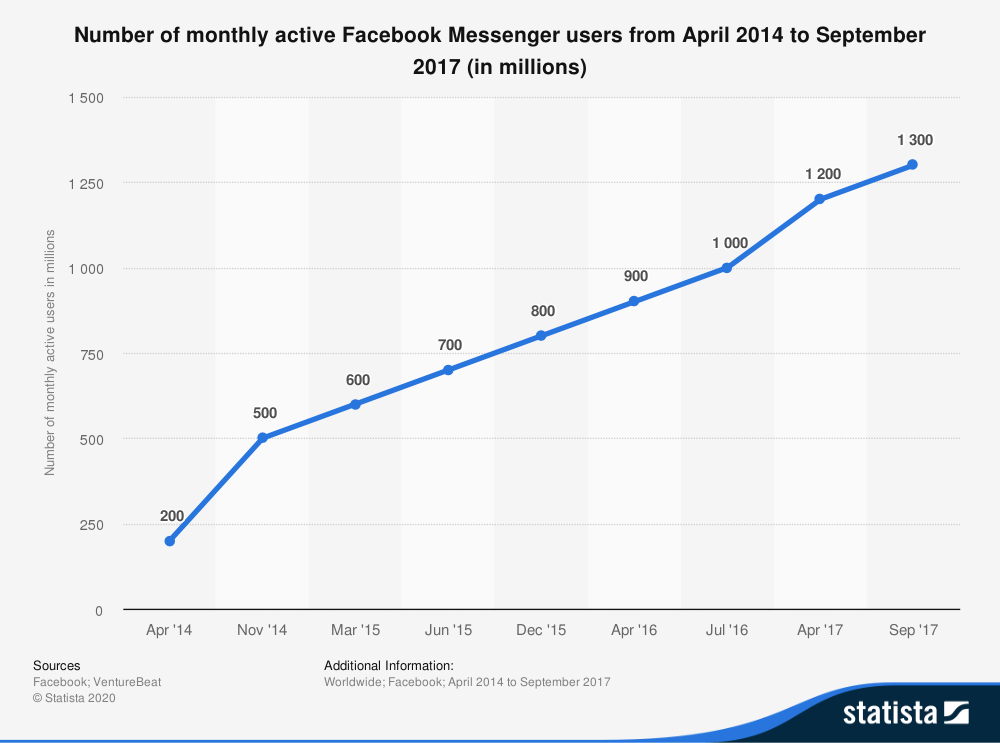
\includegraphics[width=17cm]{img/statistic_id417295_facebook-messenger_-number-of-monthly-active-users-2014-2017.png}
       \caption{Número de utilizadores mensais do \textit{Facebook Messenger} entre abril de 2014 e setembro de 2017. \cite{messenger_monthly_users}}
       \label{graph:messenger_monthly_active}
   \end{center}
\end{figure}

Já quanto ao número de \textit{downloads} feitos no \textit{Google Play}, obtidos em \cite{messenger_downloads_android}:

\begin{itemize}
   \item \textbf{Número total de \textit{downloads}}: 4 522 774 353
   \item \textbf{Número médio de \textit{downloads} diários}: 1 521 075
\end{itemize}


\subsection{Comparação}
Como já foi explicado, o \textit{Signal} não publica quaisquer dados de utilização dos seus utilizadores, o que torna difícil fazer comparação com outras aplicações do mesmo tipo. Contudo, há empresas que se "dedicam" a recolher esse tipo de dados de outras formas, como é o caso da \textit{SimilarWeb}, que obtém grande parte dos dados que disponibiliza aos seus utilizadores através de parcerias com operadores de \textit{internet} (explicação mais detalhada de como isso é feito em \cite{first_report}) por exemplo. \cite{similar_web_methodology}
Desta forma, na figura \ref{graph:all_monthly_active} é apresentado um gráfico do número de utilizadores ativos em cada uma das três aplicações analisadas nos Estados Unidos da América, em ambiente Android (aplicações obtidas no \textit{Google Play}).

\begin{figure}[H]
   \begin{center}
       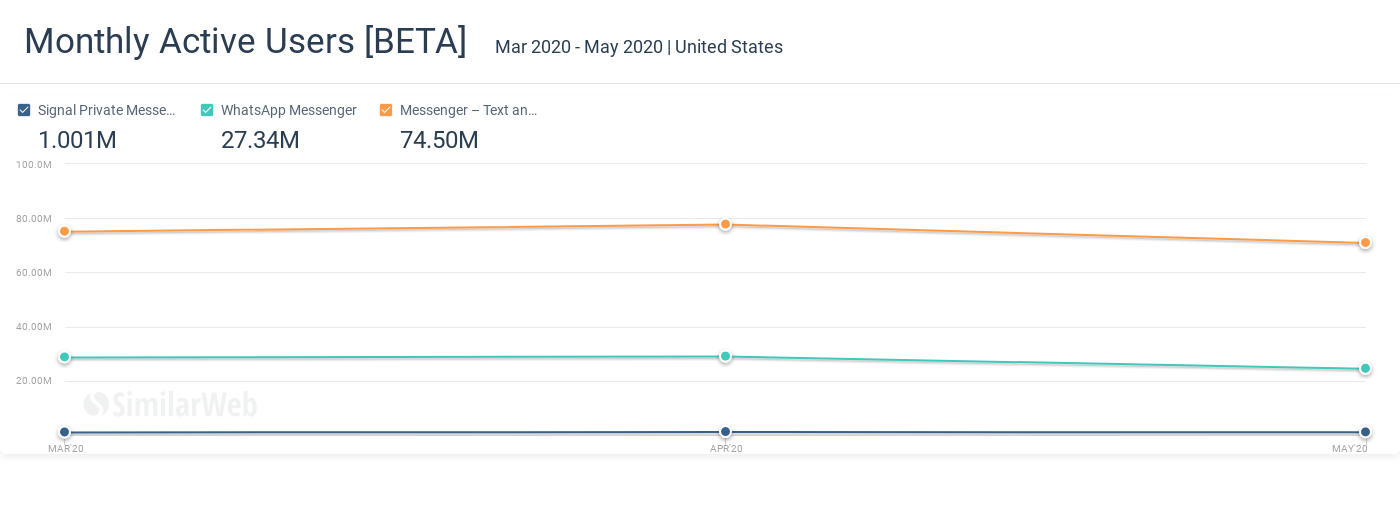
\includegraphics[width=17cm]{img/Monthly Active Users [BETA] (2020_06_10_2020_06_10).png}
       \caption{Número de utilizadores mensais do \textit{Signal}, \textit{WhatsApp} e \textit{Facebook Messenger} entre março e maio de 2020 nos Estados Unidos da América, em ambiente android. \cite{all_monthly_users}}
       \label{graph:all_monthly_active}
   \end{center}
\end{figure}

% meter gráficos de downloads (fazer em matlab ou smth)
